% This file was created by tikzplotlib v0.8.7.
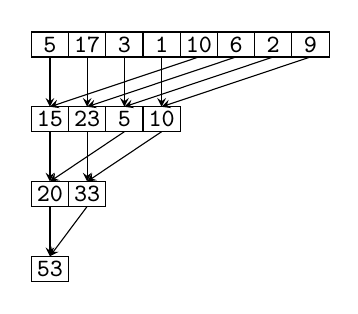
\begin{tikzpicture}

\definecolor{color0}{rgb}{1,0.498039215686275,0.0549019607843137}
\definecolor{color1}{rgb}{0.172549019607843,0.627450980392157,0.172549019607843}

\begin{axis}[
legend cell align={left},
legend style={fill opacity=0.8, draw opacity=1, text opacity=1, draw=white!80.0!black},
tick align=outside,
tick pos=left,
x grid style={white!69.01960784313725!black},
xlabel={Runtime (s)},
xmin=-9.5, xmax=19.5,
xtick style={color=black},
ymin=-3, ymax=15,
hide axis
]

% Array of 8
% \draw (1,10) rectangle (17,11);
\draw (1,10) rectangle (3,11);
\node[] at (axis cs: 2,10.5) {\small\texttt{5}};
\draw[->,>=stealth] (2,10) to (2, 8);
\draw (3,10) rectangle (5,11);
\node[] at (axis cs: 4,10.5) {\small\texttt{17}};
\draw[->,>=stealth] (4,10) to (4, 8);
\draw (5,10) rectangle (7,11);
\node[] at (axis cs: 6,10.5) {\small\texttt{3}};
\draw[->,>=stealth] (6,10) to (6, 8);
\draw (7,10) rectangle (9,11);
\node[] at (axis cs: 8,10.5) {\small\texttt{1}};
\draw[->,>=stealth] (8,10) to (8, 8);

\draw (9,10) rectangle (11,11);
\node[] at (axis cs: 10,10.5) {\small\texttt{10}};
\draw[->,>=stealth] (10,10) to (2,8);
% \draw[->,>=stealth] plot [smooth,tension=1] coordinates {(10,10) (8.333,9.333) (4.333,8.666) (2,8)};
\draw (11,10) rectangle (13,11);
\node[] at (axis cs: 12,10.5) {\small\texttt{6}};
\draw[->,>=stealth] (12,10) to (4,8);
% \draw[->,>=stealth] plot [smooth,tension=1] coordinates {(12,10) (10.333,9.333) (6.333,8.666) (4,8)};
\draw (13,10) rectangle (15,11);
\node[] at (axis cs: 14,10.5) {\small\texttt{2}};
\draw[->,>=stealth] (14,10) to (6,8);
% \draw[->,>=stealth] plot [smooth,tension=1] coordinates {(14,10) (12.333,9.333) (8.333,8.666) (6,8)};
\draw (15,10) rectangle (17,11);
\node[] at (axis cs: 16,10.5) {\small\texttt{9}};
\draw[->,>=stealth] (16,10) to (8,8);
% \draw[->,>=stealth] plot [smooth,tension=1] coordinates {(16,10) (14.333,9.333) (10.333,8.666) (8,8)};


% Array of 4
\draw (1,7) rectangle (3,8);
\node[] at (axis cs: 2,7.5) {\small\texttt{15}};
\draw[->,>=stealth] (2,7) to (2, 5);
\draw (3,7) rectangle (5,8);
\node[] at (axis cs: 4,7.5) {\small\texttt{23}};
\draw[->,>=stealth] (4,7) to (4, 5);
\draw (5,7) rectangle (7,8);
\node[] at (axis cs: 6,7.5) {\small\texttt{5}};
\draw[->,>=stealth] (6,7) to (2,5);
% \draw[->,>=stealth] plot [smooth,tension=1] coordinates {(6,7) (5.333,6.333) (3.333,5.666) (2,5)};
\draw (7,7) rectangle (9,8);
\node[] at (axis cs: 8,7.5) {\small\texttt{10}};
\draw[->,>=stealth] (8,7) to (4,5);
% \draw[->,>=stealth] plot [smooth,tension=1] coordinates {(8,7) (7.333,6.333) (5.333,5.666) (4,5)};


% Array of 2
\draw (1,4) rectangle (3,5);
\node[] at (axis cs: 2,4.5) {\small\texttt{20}};
\draw[->,>=stealth] (2,4) to (2, 2);
\draw (3,4) rectangle (5,5);
\node[] at (axis cs: 4,4.5) {\small\texttt{33}};
\draw[->,>=stealth] (4,4) to (2, 2);
% \draw[->,>=stealth] plot [smooth,tension=1] coordinates {(4,4) (3.666,3.333) (2.666,2.666) (2,2)};

% Array of 1
\draw (1,1) rectangle (3,2);
\node[] at (axis cs: 2,1.5) {\small\texttt{53}};


% \draw[->,>=stealth] (-1.5,7) to[bend right=-60] (2.5, 7);
% \draw[->,>=stealth] (8.5,7) to[bend right=-60] (12.5, 7);

% \draw[->,>=stealth] (1.5,1) to[bend right=-60] (-2.5, 1);
% \draw[->,>=stealth] (11.5,1) to[bend right=-60] (7.5, 1);

% \addplot [color0, forget plot]
% table {%
% 0.009462 0.925
% 0.009462 1.075
% };
\end{axis}

\end{tikzpicture}
